
\documentclass{article}
\usepackage{amsmath}
\usepackage{graphicx}
\usepackage{subcaption}
\usepackage{array}
\usepackage[margin=1.0in]{geometry}
\usepackage[utf8]{inputenc}
\usepackage{hyperref}
\usepackage{float}

\begin{document}

\begin{titlepage}
    \centering
    \vspace*{2cm}
    {\Huge\bfseries Report\par}
    \vspace{2cm}
    {\Large\itshape Homework 2\par}
    \vspace{0.5cm}
    {\large\itshape Goal: Image Classification with CNN for a self driving car in OpenAI Gym\par}
    \vfill
    {\Large Andrea Massignan\par}
    {\Large 1796802\par}
    \vfill
    \href{https://github.com/duchannes19/Homework-2}{GitHub Repository}
\end{titlepage}

\section{Introduction}

In this homework assignment, the objective is to address the image classification problem focused on understanding the behavior of a racing car within the OpenAI Gym environment. The task involves classifying 96x96 color images, each corresponding to one of the five distinct actions available for controlling the car.

\section{Methodology}

The image classification task is addressed using convolutional neural network (CNN) models. The CNN architecture is implemented using the Keras API with a TensorFlow backend. The models are trained on the labeled training set and evaluated on the separate test set.
\newline
\newline
Here is how I approached the problem.

\section{Data Preprocessing}

In this section, I describe the data preprocessing steps implemented for training a Convolutional Neural Network (CNN) to classify images in the context of a self-driving car simulation. The preprocessing pipeline makes so that the data is appropriately formatted and augmented for robust training while maintaining consistency for validation.
\\\\
The dataset was split into a training set and a validation set, each set contains images organized into subdirectories corresponding to their respective classes.
\\\\
To handle the variability in image sizes and ensure compatibility with the CNN architecture, all images were resized to a target size of \(96 \times 96\) pixels. The images were loaded in RGB format, which preserves the color information for classification. The batch size was set to 64.

\subsection{Training Data Augmentation}

To enhance the generalizability of the model, data augmentation was applied to the training set using the \texttt{ImageDataGenerator} class from Keras. Augmentation techniques included:

\begin{itemize}
    \item \textbf{Rescaling}: All pixel values were normalized to the range [0, 1] by dividing by 255.
    \item \textbf{Zooming}: A random zoom range of 10\% was applied to simulate variations in image scale.
    \item \textbf{Shifting}: Random shifts up to 10\% in both width and height directions were introduced.
    \item \textbf{Horizontal Flipping}: Random horizontal flips were applied to account for variations in vehicle orientation.
    \item \textbf{Rotation}: Images were randomly rotated within a range of 20 degrees.
    \item \textbf{Shearing}: Shear transformations with a range of 10\% were used to modify the image perspective slightly.
    \item \textbf{Fill Mode}: When augmentations resulted in empty areas, pixels were filled using the nearest pixel values.
\end{itemize}

\subsection{Validation Data Processing}

For the validation set, data augmentation was intentionally omitted to preserve the original data distribution and provide an unbiased evaluation of the model's performance. The images in this set were rescaled to the range [0, 1].

\subsection{Data Generators}

The training and validation data were loaded using generators, which allow for efficient batch processing:
\begin{itemize}
    \item \texttt{train\_generator}: Reads the augmented training images and their corresponding labels in batches.
    \item \texttt{validation\_generator}: Loads validation images without augmentation for consistent evaluation.
\end{itemize}

\subsection{Dataset Overview}

The preprocessing pipeline gave this insights into the dataset:
\begin{itemize}
    \item Input images have a shape of \(96 \times 96 \times 3\), where the dimensions correspond to height, width, and color channels, respectively.
    \item The training set comprises \texttt{train\_generator.n} samples distributed across \texttt{train\_generator.num\_classes} classes.
    \item The validation set consists of \texttt{validation\_generator.n} samples spanning the same number of classes as the training set.
    \item The class names, derived from the directory structure, \\ are: \texttt{train\_generator.class\_indices.keys()}.
\end{itemize}

\section{Class Distribution Analysis}

To better understand the distribution of samples across different classes in the training dataset, I performed an analysis of the class distribution. Uneven distribution of samples among classes, often referred to as class imbalance, can negatively affect the training process, leading to biased predictions. This analysis helps identify potential imbalances that may require corrective measures.
\\\\
The number of samples per class was computed using the \texttt{train\_generator.classes} attribute, which provides the class labels for all images in the training set. The class names were retrieved from the generator's \texttt{class\_indices} attribute. A bar plot was generated to visualize the distribution.

\subsection{Visualization of Class Distribution}

The figure in the next page displays the class distribution in the training set. Each bar corresponds to a class, and its height represents the number of samples available for that class. The visualization was created using \texttt{matplotlib} this way:

\begin{itemize}
    \item The total count of samples per class was calculated by summing the occurrences of each class label.
    \item A bar chart was plotted, where the x-axis represents the class names, and the y-axis represents the number of samples.
\end{itemize}

\begin{figure}[h!]
    \centering
    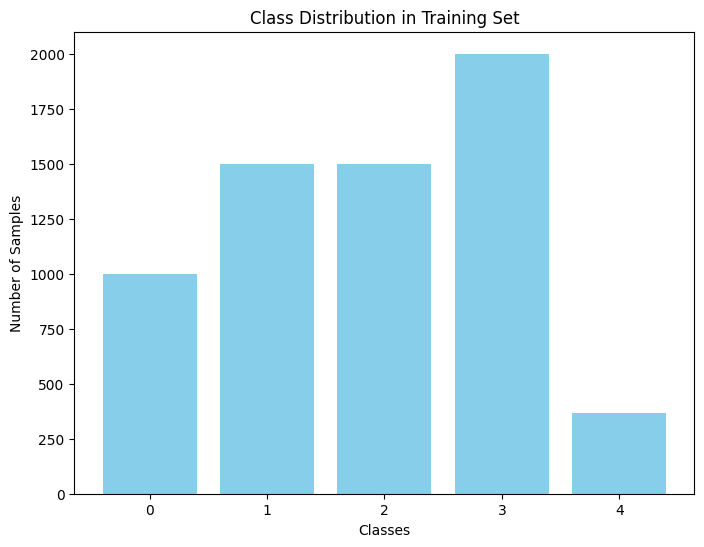
\includegraphics[width=0.8\textwidth]{class_distribution.png}
    \caption{Class distribution in the training set.}
    \label{fig:class_distribution}
\end{figure}

\newpage

\subsection{Observations}

The class distribution in the training dataset, as depicted in Figure~\ref{fig:class_distribution}, reveals variability in the representation of different classes:

\begin{itemize}
    \item \textbf{Class 3} is the most represented, with approximately 2000 samples.
    \item \textbf{Classes 1 and 2} are moderately represented, each containing around 1500 samples.
    \item \textbf{Class 0} has fewer samples, with just above 1000 samples.
    \item \textbf{Class 4} is significantly underrepresented, containing fewer than 500 samples.
\end{itemize}

\noindent
This distribution indicates an imbalance in the dataset, with Class 4 being particularly underrepresented and Class 3 dominating the dataset. Such imbalances may lead to biased model performance, favoring overrepresented classes and leading to overfitting

\subsection{Creating Separate Generators for Minority Classes}

To address the observed class imbalance in the dataset, I implemented a strategy to augment the minority classes separately. This approach focuses on increasing the representation of the underrepresented classes in the training data, and this is done by re-applying the augmentation techniques to the images in these classes. The goal is to balance the class distribution and improve the model's ability to generalize across all classes.

\subsubsection{Target Classes and Data Augmentation}

The classes identified as minority classes in the dataset were \textbf{Class 0} and \textbf{Class 4}.
\\\\
The augmentation techniques applied to the minority classes included \textbf{normalizing} pixel values to the range [0, 1], applying random \textbf{zooms} up to 20\% to simulate changes in scale, introducing random \textbf{horizontal and vertical shifts} up to 20\%, randomly \textbf{flipping} images horizontally, performing random \textbf{rotations} up to 30 degrees, applying \textbf{shear transformations} up to 20\%, and filling any empty areas created during transformations using the \textbf{nearest pixel values}.

\subsubsection{Implementation}

Separate generators were created for the minority classes using the \texttt{ImageDataGenerator} class, targeting their respective directories within the training dataset. Only the directories corresponding to the minority classes (\texttt{Class 0} and \texttt{Class 4}) were processed. Each generator was configured to shuffle the data and output augmented samples in batches of 64 images, resized to \(96 \times 96\) pixels.

\subsubsection{Outcome}

For each minority class, a generator was successfully created, provided that the class directory existed in the training dataset. If a directory was not found, the process skipped that class with a notification.

\subsection{Computing Class Weights}

To further address the issue of class imbalance in the training dataset, class weights were computed. Class weights help the model prioritize learning from underrepresented classes by assigning higher importance to their corresponding loss during training. This ensures that the model does not become biased toward overrepresented classes.

\subsubsection{Methodology}

The class weights were calculated using the \texttt{class\_weight.compute\_class\_weight} function from \texttt{sklearn.utils}. This function computes the weights inversely proportional to the frequency of each class, ensuring that all classes are equally considered during training. The computation steps are as follows:
\begin{itemize}
    \item The unique class labels were extracted from \texttt{train\_generator.classes}.
    \item The class weights were calculated using the formula:
    \[
    \text{weight}_{i} = \frac{\text{total samples}}{\text{number of classes} \times \text{samples in class}_{i}}
    \]
    \item The weights were converted into a dictionary for easy integration during model training.
\end{itemize}

\subsubsection{Results}

The computed class weights were:
\\\\
\textbf{Class Weights:} \texttt{class\_weights\_dict}
\\\\
These weights assign higher values to underrepresented classes (e.g., Class 4), while overrepresented classes (e.g., Class 3) receive lower weights. 

\subsubsection{Significance}

By incorporating class weights during model training, the loss function will penalize misclassifications of underrepresented classes more heavily. This adjustment should help to improve the model's performance on minority classes without artificially modifying the dataset or oversampling.
\\\\
In this case specifically, the class weights are the following:

\begin{verbatim}
Class Weights: {0: 1.2738, 1: 0.8492, 2: 0.8492, 3: 0.6369, 4: 3.4520}
\end{verbatim}

\subsection{Combining Original and Augmented Generators}

To ensure a comprehensive dataset for training, the original training generator was combined with the augmented generators created for the minority classes. This approach effectively merges the balanced representation from the augmentation process with the natural variability of the original dataset, improving the overall robustness of the model.

\subsubsection{Methodology}

The combination was implemented using the \texttt{itertools.chain} function, which allows for the seamless concatenation of multiple generators. These steps were performed:
\begin{itemize}
    \item The original training generator (\texttt{train\_generator}) was combined with the augmented generators created for the minority classes.
    \item A wrapper generator function, \texttt{combined\_generator}, was defined to yield data batches from the combined generator.
    \item The iterator for the combined generator was reset to ensure a clean start during training.
\end{itemize}

\subsubsection{Advantages}

The combined generator should offer:
\begin{itemize}
    \item \textbf{Increased Diversity}: Combines naturally occurring samples with augmented samples, providing more diverse training data.
    \item \textbf{Class Balance}: Includes additional samples for minority classes, mitigating class imbalance.
    \item \textbf{Seamless Integration}: Maintains the batch-wise data flow required for efficient training in deep learning frameworks.
\end{itemize}

\section{Model Definition}

In this section, I define two Convolutional Neural Network (CNN) architectures, thought for the image classification task: a \texttt{First CNN} and a \texttt{Second CNN}. Both models leverage multiple convolutional blocks to extract hierarchical features from input images, followed by dense layers for classification. These architectures differ in their complexity, optimization strategies, and regularization techniques.

\subsection{First CNN Architecture}

The \texttt{First CNN} model is a sequential architecture consisting of three convolutional blocks, each followed by pooling and dropout layers to reduce overfitting. The key components are as follows:
\begin{itemize}
    \item \textbf{First Convolutional Block:} Includes two convolutional layers with 32 filters of size \(3 \times 3\) and ReLU activation, followed by max pooling (\(2 \times 2\)) and dropout (30\%).
    \item \textbf{Second Convolutional Block:} Contains two convolutional layers with 64 filters of size \(3 \times 3\) and ReLU activation, followed by max pooling and dropout (30\%).
    \item \textbf{Third Convolutional Block:} Comprises two convolutional layers with 128 filters of size \(3 \times 3\) and ReLU activation, followed by max pooling and dropout (40\%).
    \item \textbf{Dense Layers:} A fully connected layer with 512 units and ReLU activation is followed by a 50\% dropout layer. The output layer uses a softmax activation to classify the images into the desired number of classes.
\end{itemize}

The model is compiled with the RMSprop optimizer and a learning rate of 0.001, employing categorical cross-entropy as the loss function. This architecture serves as a strong baseline for the task.

\subsection{Second CNN Architecture}

The \texttt{Second CNN} model builds on the \texttt{First CNN} architecture by incorporating several enhancements aimed at improving performance:
\begin{itemize}
    \item \textbf{Batch Normalization:} Added after each convolutional layer to stabilize learning and accelerate convergence.
    \item \textbf{Leaky ReLU Activation:} Replaces the standard ReLU activation, allowing for small gradients even for negative inputs, which prevents neuron "dying."
    \item \textbf{Global Average Pooling:} Used instead of flattening after the convolutional blocks, reducing the risk of overfitting by minimizing the number of parameters.
    \item \textbf{Kernel Regularization:} A regularization term (\(L2\)) is applied to the dense layer to further mitigate overfitting.
    \item \textbf{Adam Optimizer:} A more advanced optimization algorithm with a learning rate of 0.0001, offering adaptive learning rates for better convergence.
\end{itemize}

The architecture retains three convolutional blocks but augments each with the additional features described above. Dropout is applied at various points to introduce regularization.

\section{Model Training}

The training phase involves optimizing the \texttt{First CNN} and \texttt{Second CNN} models using the preprocessed dataset and the combined generators. This section outlines the training strategy, including the use of callbacks for dynamic learning rate adjustment, early stopping, and model checkpointing.

\subsection{Callbacks}

To monitor and enhance the training process, three key callbacks were employed:
\begin{itemize}
    \item \textbf{Early Stopping:} This callback monitors the validation loss and stops training if there is no improvement for 10 consecutive epochs. Additionally, it restores the model weights corresponding to the best validation performance to prevent overfitting.
    \item \textbf{ReduceLROnPlateau:} This callback reduces the learning rate by a factor of 0.2 if the validation loss does not improve for 3 consecutive epochs, ensuring gradual convergence.
    \item \textbf{Model Checkpoint:} The best model, based on validation accuracy, is saved to a file (\texttt{models/best\_model.keras}) during training. This ensures the best performing model is preserved even if training is interrupted.
\end{itemize}

\subsection{Training Configuration}

The training process was configured with this parameters:
\begin{itemize}
    \item \textbf{Epochs:} Both models were trained for up to 100 epochs, with early stopping enabled to terminate training when no further improvement is observed.
    \item \textbf{Steps Per Epoch:} Calculated as the total number of samples in the training set divided by the batch size, rounded up to ensure all samples are utilized.
    \item \textbf{Validation Steps:} Similarly, computed for the validation set.
    \item \textbf{Class Weights:} The previously computed class weights were applied to emphasize learning from underrepresented classes.
\end{itemize}

If the training process was interrupted manually (e.g., via a keyboard interrupt), the models were saved at their current state to avoid loss of progress.

\subsection{Model Saving}

Upon completion of the training, the final versions of both models were saved to disk for future use:
\begin{itemize}
    \item \textbf{First CNN:} Saved as \texttt{models/final\_model\_deep.keras}.
    \item \textbf{Second CNN:} Saved as \texttt{models/final\_model\_improved.keras}.
\end{itemize}

\section{Creating and Evaluating the Combined Model}

To leverage the strengths of both the \texttt{First CNN} and \texttt{Second CNN} architectures, a combined model was created by averaging the predictions of the two individual models.

\subsection{Architecture of the Combined Model}

The combined model was constructed as follows:
\begin{itemize}
    \item \textbf{Input Layer:} A single input layer was defined with the shape matching the input dimensions of both \texttt{First CNN} and \texttt{Second CNN}. To ensure compatibility, the input shapes of the two models were verified to be identical.
    \item \textbf{Predictions from Individual Models:} The predictions from both \texttt{First CNN} and \texttt{Second CNN} were obtained by passing the input layer through each pre-trained model.
    \item \textbf{Averaging Layer:} The outputs of the two models were combined using an averaging layer, which computes the element-wise mean of the predictions. This ensemble strategy smooths out individual model errors and improves robustness.
    \item \textbf{Output Layer:} The averaged predictions serve as the final output of the combined model, representing the probabilities for each class.
\end{itemize}

\subsection{Compilation and Saving}

The combined model was compiled with this configuration:
\begin{itemize}
    \item \textbf{Loss Function:} Categorical cross-entropy was used as the loss function, consistent with the individual models.
    \item \textbf{Optimizer:} The Adam optimizer with a learning rate of 0.0001 was selected for its adaptive learning capabilities.
    \item \textbf{Metrics:} Accuracy was used as the primary evaluation metric.
\end{itemize}

\subsection{Model Evaluation Summary}

The results, including the loss, accuracy, and classification metrics, are summarized here:

\subsubsection{Validation Metrics}

\begin{table}[h!]
    \centering
    \begin{tabular}{|c|c|c|}
        \hline
        \textbf{Model} & \textbf{Loss} & \textbf{Accuracy} \\
        \hline
        First CNN & 1.3909 & 0.6162 \\
        Second CNN & 1.3409 & 0.6744 \\
        Combined CNN & 1.3079 & 0.7159 \\
        \hline
    \end{tabular}
    \caption{Validation Loss and Accuracy for All Models}
    \label{tab:validation_metrics_summary}
\end{table}

\subsubsection{Classification Reports}

The detailed classification reports for each model, which provide precision, recall, F1-score, and support for all classes, are presented in the following tables.

\begin{table}[h!]
    \centering
    \begin{tabular}{cc}
        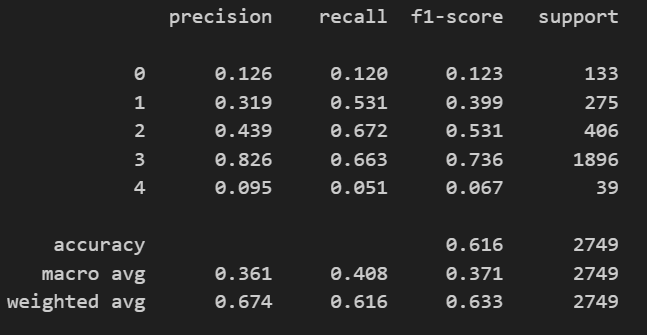
\includegraphics[width=0.45\textwidth]{DeepCNN.png} &
        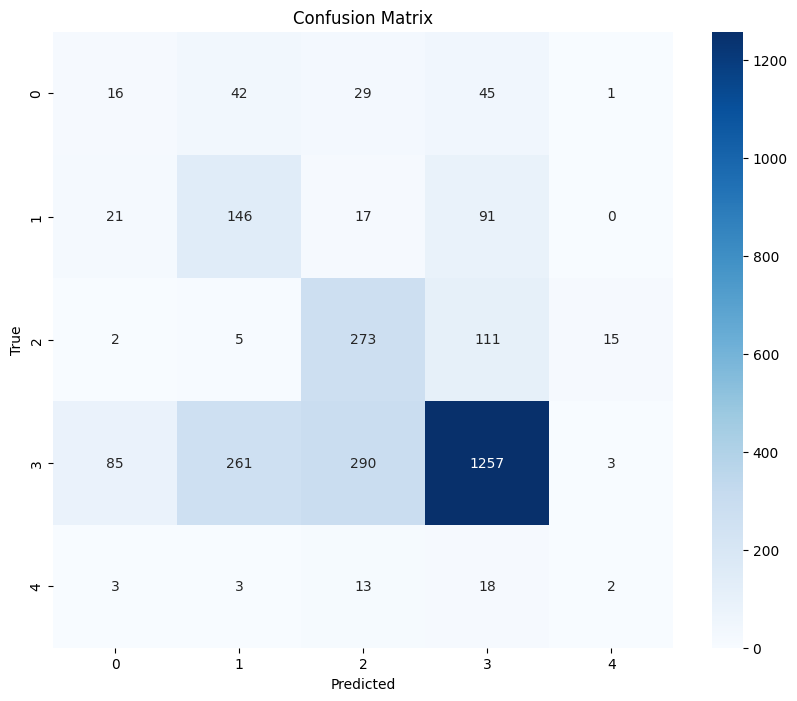
\includegraphics[width=0.45\textwidth]{deep_cnn_cf.png} \\
        \multicolumn{1}{c}{\textbf{Classification Report}} &
        \multicolumn{1}{c}{\textbf{Confusion Matrix}} \\
    \end{tabular}
    \caption{Evaluation Metrics for the First CNN}
    \label{tab:deep_cnn_metrics}
\end{table}
\vspace{1cm}
\begin{table}[h!]
    \centering
    \begin{tabular}{cc}
        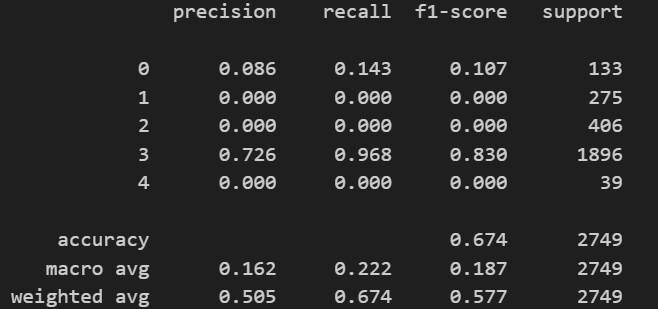
\includegraphics[width=0.45\textwidth]{ImprovedCNN.png} &
        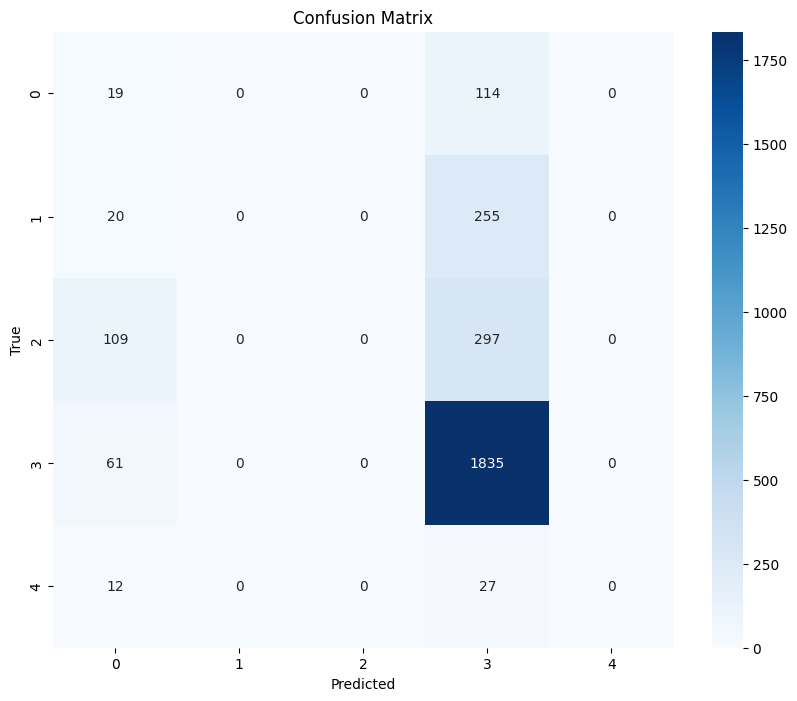
\includegraphics[width=0.45\textwidth]{improved_cnn_cf.png} \\
        \multicolumn{1}{c}{\textbf{Classification Report}} &
        \multicolumn{1}{c}{\textbf{Confusion Matrix}} \\
    \end{tabular}
    \caption{Evaluation Metrics for Second CNN}
    \label{tab:improved_cnn_metrics}
\end{table}
\vspace{1cm}
\begin{table}[h!]
    \centering
    \begin{tabular}{cc}
        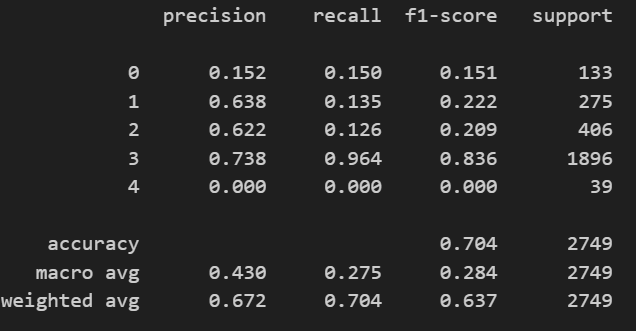
\includegraphics[width=0.45\textwidth]{CombinedCNN.png} &
        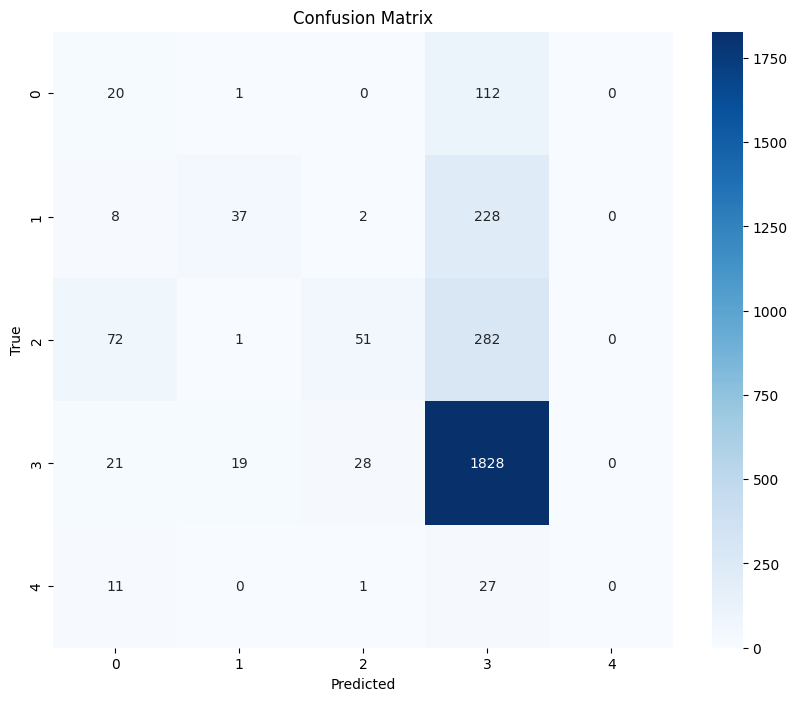
\includegraphics[width=0.45\textwidth]{combined_cnn_cf.png} \\
        \multicolumn{1}{c}{\textbf{Classification Report}} &
        \multicolumn{1}{c}{\textbf{Confusion Matrix}} \\
    \end{tabular}
    \caption{Evaluation Metrics for the Combined CNN}
    \label{tab:combined_cnn_metrics}
\end{table}

\newpage

\subsubsection{Observations}

\begin{itemize}
    \item The \textbf{First CNN} achieved the lowest accuracy (61.62\%) and the highest loss (1.3909), indicating its comparatively limited capacity to generalize on the validation set.
    \item The \textbf{Second CNN} outperformed the \texttt{First CNN}, achieving an accuracy of 67.44\% and a slightly lower loss of 1.3409, highlighting the benefits of batch normalization, Leaky ReLU, and regularization techniques.
    \item The \textbf{Combined Model} achieved the highest validation accuracy of 71.59\%, with the lowest loss of 1.3079, demonstrating its effectiveness in leveraging the strengths of both \texttt{First CNN} and \texttt{Second CNN}.
\end{itemize}

\subsection{Model Deployment in Gymnasium Environment}

The best-performing model was deployed in the \texttt{CarRacing-v3} environment from Gymnasium. The goal was to control the car using the model's predictions, mapping the classification outputs to predefined continuous actions, even though it was an optional task.

\subsubsection{Environment Setup}

The environment was initialized using this parameters:
\begin{itemize}
    \item \textbf{Domain Randomization:} Disabled to maintain consistent environmental conditions.
    \item \textbf{Render Mode:} Set to \texttt{rgb\_array} to enable observation rendering.
\end{itemize}

\subsubsection{Predefined Actions}
A set of continuous actions was predefined to control the car based on the model's predictions. These actions include no action, steering left, steering right, accelerating, and braking.

\subsubsection{Performance in the Environment}

The car was controlled using this approach:
\begin{itemize}
    \item Observations from the environment were preprocessed and fed into the trained model.
    \item The model's predicted class was mapped to a corresponding predefined action.
    \item The environment was stepped with the selected action until the episode terminated.
\end{itemize}

\noindent
The interaction with the environment was recorded as a video for further analysis and demonstration purposes.

\subsection{Results}

Alas, the model was not able to control the car effectively in the Gymnasium environment. The car often veered off the track or failed to navigate turns, indicating a lack of robustness in the model's predictions. The performance was inconsistent, with occasional successes but frequent failures in controlling the car effectively. I'm afraid this is due to the overfitting, which even if mitigated by the ensemble model, was still present in the final model, due to the lack of data and the class imbalance.

\section{Reinforcement Learning Approach}

An optional component of this project involved implementing a reinforcement learning (RL) approach to solve the \texttt{CarRacing-v3} task using a Deep Q-Network (DQN) agent. This approach was designed to train a neural network to autonomously control the car by interacting with the environment and learning from its actions. However, due to hardware limitations and the extensive training time required, this component was not completed to its full extent.

\subsection{Overview of the Reinforcement Learning Approach}

The RL implementation followed a classical DQN architecture with the following elements:
\begin{itemize}
    \item \textbf{Deep Q-Network (DQN):} A convolutional neural network that predicts Q-values for a set of predefined continuous actions.
    \item \textbf{Action Space:} A set of continuous steering, gas, and brake actions was defined for controlling the car.
    \item \textbf{Replay Memory:} A memory buffer to store past experiences, which were replayed during training to stabilize learning.
    \item \textbf{Target Model Updates:} A secondary target model was used to stabilize training by providing consistent Q-value estimates.
\end{itemize}

\subsection{Implementation Details}

The implementation included utility functions for preprocessing frames, seeding randomness, and saving results, along with a configuration class to manage hyperparameters. The training loop leveraged a reward system to guide the agent's learning and included mechanisms to skip frames for efficiency. A test function was also defined to evaluate a trained model in a live environment.

\subsection{Challenges and Limitations}

These were the challenges that were encountered during the implementation:
\begin{itemize}
    \item \textbf{Hardware Constraints:} The training process requires significant computational resources due to the large state space and the need for extensive interactions with the environment.
    \item \textbf{Training Time:} DQN training is time-intensive, and achieving convergence would require a lot of time of uninterrupted computation.
    \item \textbf{Incomplete Execution:} Due to the aforementioned constraints, the RL approach was implemented but not fully executed to produce conclusive results.
\end{itemize}

\subsection{Inspired by Autonomous Networking Course}

This approach was inspired by an example presented during the \textit{Autonomous Networking} course last year. It was demonstrated the application of reinforcement learning for autonomous control tasks, which provided a foundation and inspiration for the design of this RL agent.

\subsection{Future Work}

With access to better hardware resources and more time, we could improve the implementation, for example:
\begin{itemize}
    \item Full training and testing of the DQN agent to validate its performance in the \texttt{CarRacing-v3} environment.
    \item Exploration of advanced RL algorithms, such as Double DQN.
    \item Integration of domain-specific reward shaping to better guide the agent's learning process.
\end{itemize}

\section{Conclusion}

In this project, I addressed the image classification task for a self-driving car in the OpenAI Gym environment using convolutional neural networks. I implemented two CNN architectures, the \texttt{First CNN} and \texttt{Second CNN}, and combined them to create an ensemble model. The combined model achieved the highest validation accuracy of 71.59\%, outperforming the individual models. 
\\\\
However, the model's performance in the Gymnasium environment was suboptimal, indicating the need for further improvements to enhance robustness and generalization. 
\\\\
The reinforcement learning approach using a DQN agent was partially implemented but not fully executed due to hardware constraints and training time limitations. Future work could focus on completing the RL implementation and exploring advanced algorithms to improve the agent's performance.

\end{document}